\documentclass{beamer}
\usepackage{amsmath}
\usepackage[latin1]{inputenc}
\usefonttheme[onlylarge]{structurebold}
\setbeamerfont*{frametitle}{size=\normalsize,series=\bfseries}
\setbeamertemplate{navigation symbols}{}
\usetheme{Goettingen}
\defbeamertemplate{itemize item}{checkbox}{\Square}
\defbeamertemplate{itemize item}{checked}{\Square\llap\CheckmarkBold}

\title[Lab Meeting III]{Lab Meeting III}
\author{Carles Boix}
\begin{document}

\begin{frame}
    \begin{center}
        {\large \textsc{Last Week (11/18):}}
    \end{center}
    \begin{figure}[ht!]
        \centering
        \includegraphics<1>[width=.9\textwidth]{FARwtdigest.png}\\
        \includegraphics<2>[width=.9\textwidth]{FARwtdigestNEB.png}
        \caption{Digest of FAR-WT}
        \label{fig:pcr}
    \end{figure}

    \begin{itemize}
        \item<2> HindIII and BamHI each cut Far1 at one site.
    \end{itemize}

\end{frame}


\begin{frame}{Selection of new primers:}
    \begin{itemize}
        \item One set with the same strategy (Enzymes NotI and XhoI).

            \begin{center}
            \scriptsize
            5'\, AATA \textbf{CTCGAG} ATGAAGACACCAACAAGAGTTTC\, 3' \\
            5'\, AATA \textbf{GCGGCCGC} CTAGAGGTTGGGAACTTCC\, 3' \\
            \end{center}
\normalsize

    \item One set for homologous recombination with the Gal vector (pMM86). Must first digest the vector with \emph{NotI} and \emph{BamHI} or a set of similar enzymes.
    \end{itemize}
\end{frame}

\begin{frame}
    \begin{figure}[ht!]
        \centering
        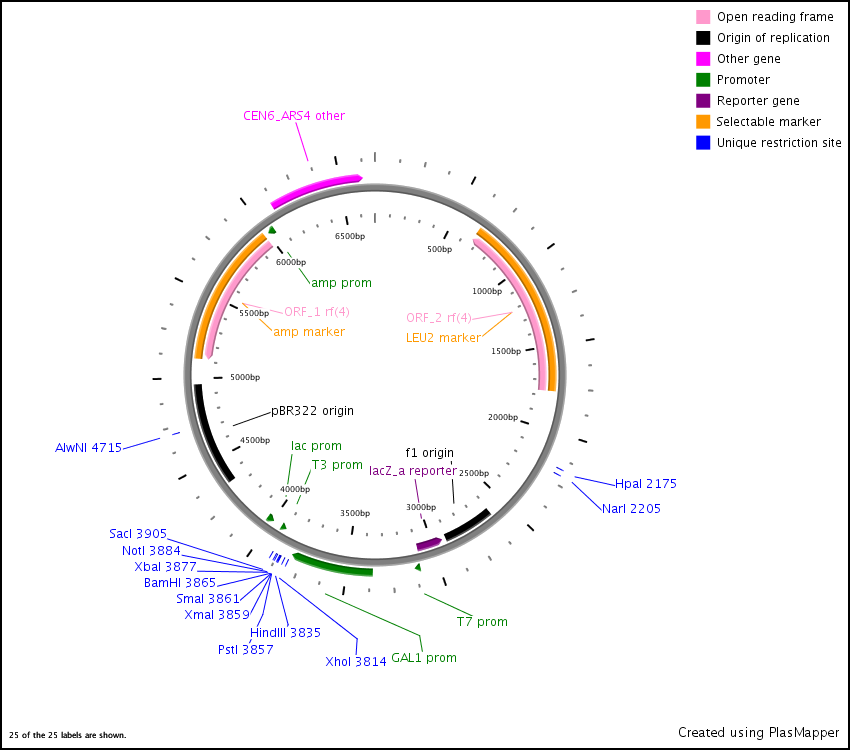
\includegraphics[width=.8\textwidth]{../Documents/plasMap_pMM86.png}
        \caption{pMM86 - GALpr vector}
        \label{fig:ligc}
    \end{figure}
\end{frame}

\begin{frame}
    \begin{figure}[ht!]
        \centering
        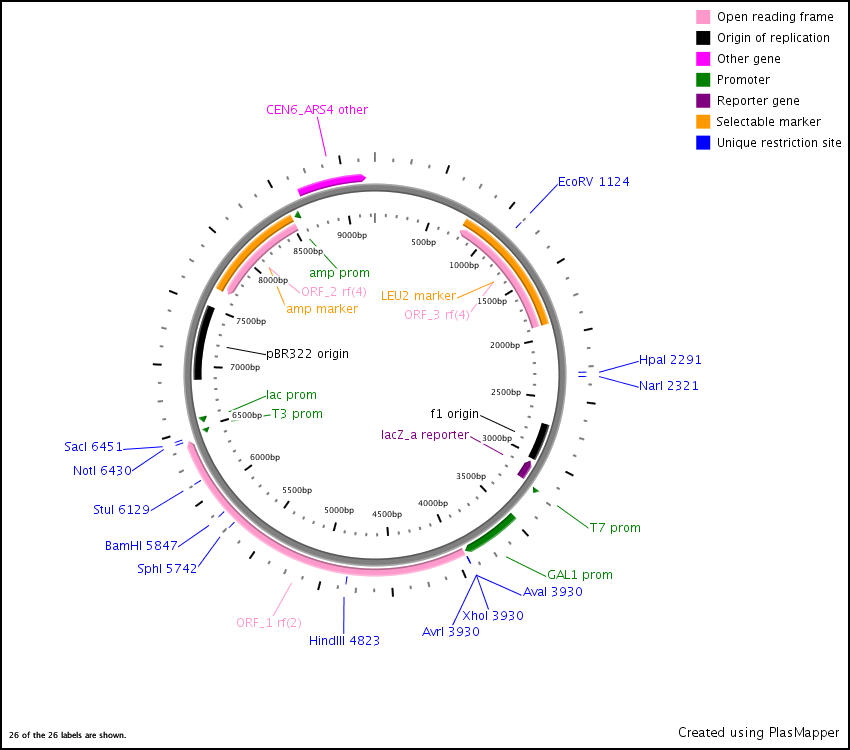
\includegraphics[width=.8\textwidth]{../Documents/plasMap_pGALFARwt.png}
        \caption{pMM86 + FAR1 by way of NotI and XhoI}
        \label{fig:ligc}
    \end{figure}
\end{frame}

\begin{frame}
    \begin{center}
        {\large \textsc{This week (11/25) and next.}}
    \end{center}
    \textbf{For restriction primers:}\\
    \begin{itemize}
        \item PCR of FAR1-22 and Genomic PCR of FAR1-WT.
        \item Digestion of PCR products and of plasmid.
        \item Ligation + Transformation into bacteria.
        \item Miniprep + digest + sequencing.
        \item Transformation into yeast.
    \end{itemize}

    \textbf{For recombination primers:}\\
    \begin{itemize}
        \item PCR of FAR1-22 and Genomic PCR of FAR1-WT.
        \item Digest of pMM86 vector.
        \item Transformation into Yeast with cut vector.
    \end{itemize}
\end{frame}

\begin{frame}{Transformation of ZEV with CORE}
    \begin{minipage}[ht!]{0.48\textwidth}
    \begin{figure}[ht!]
        \centering
        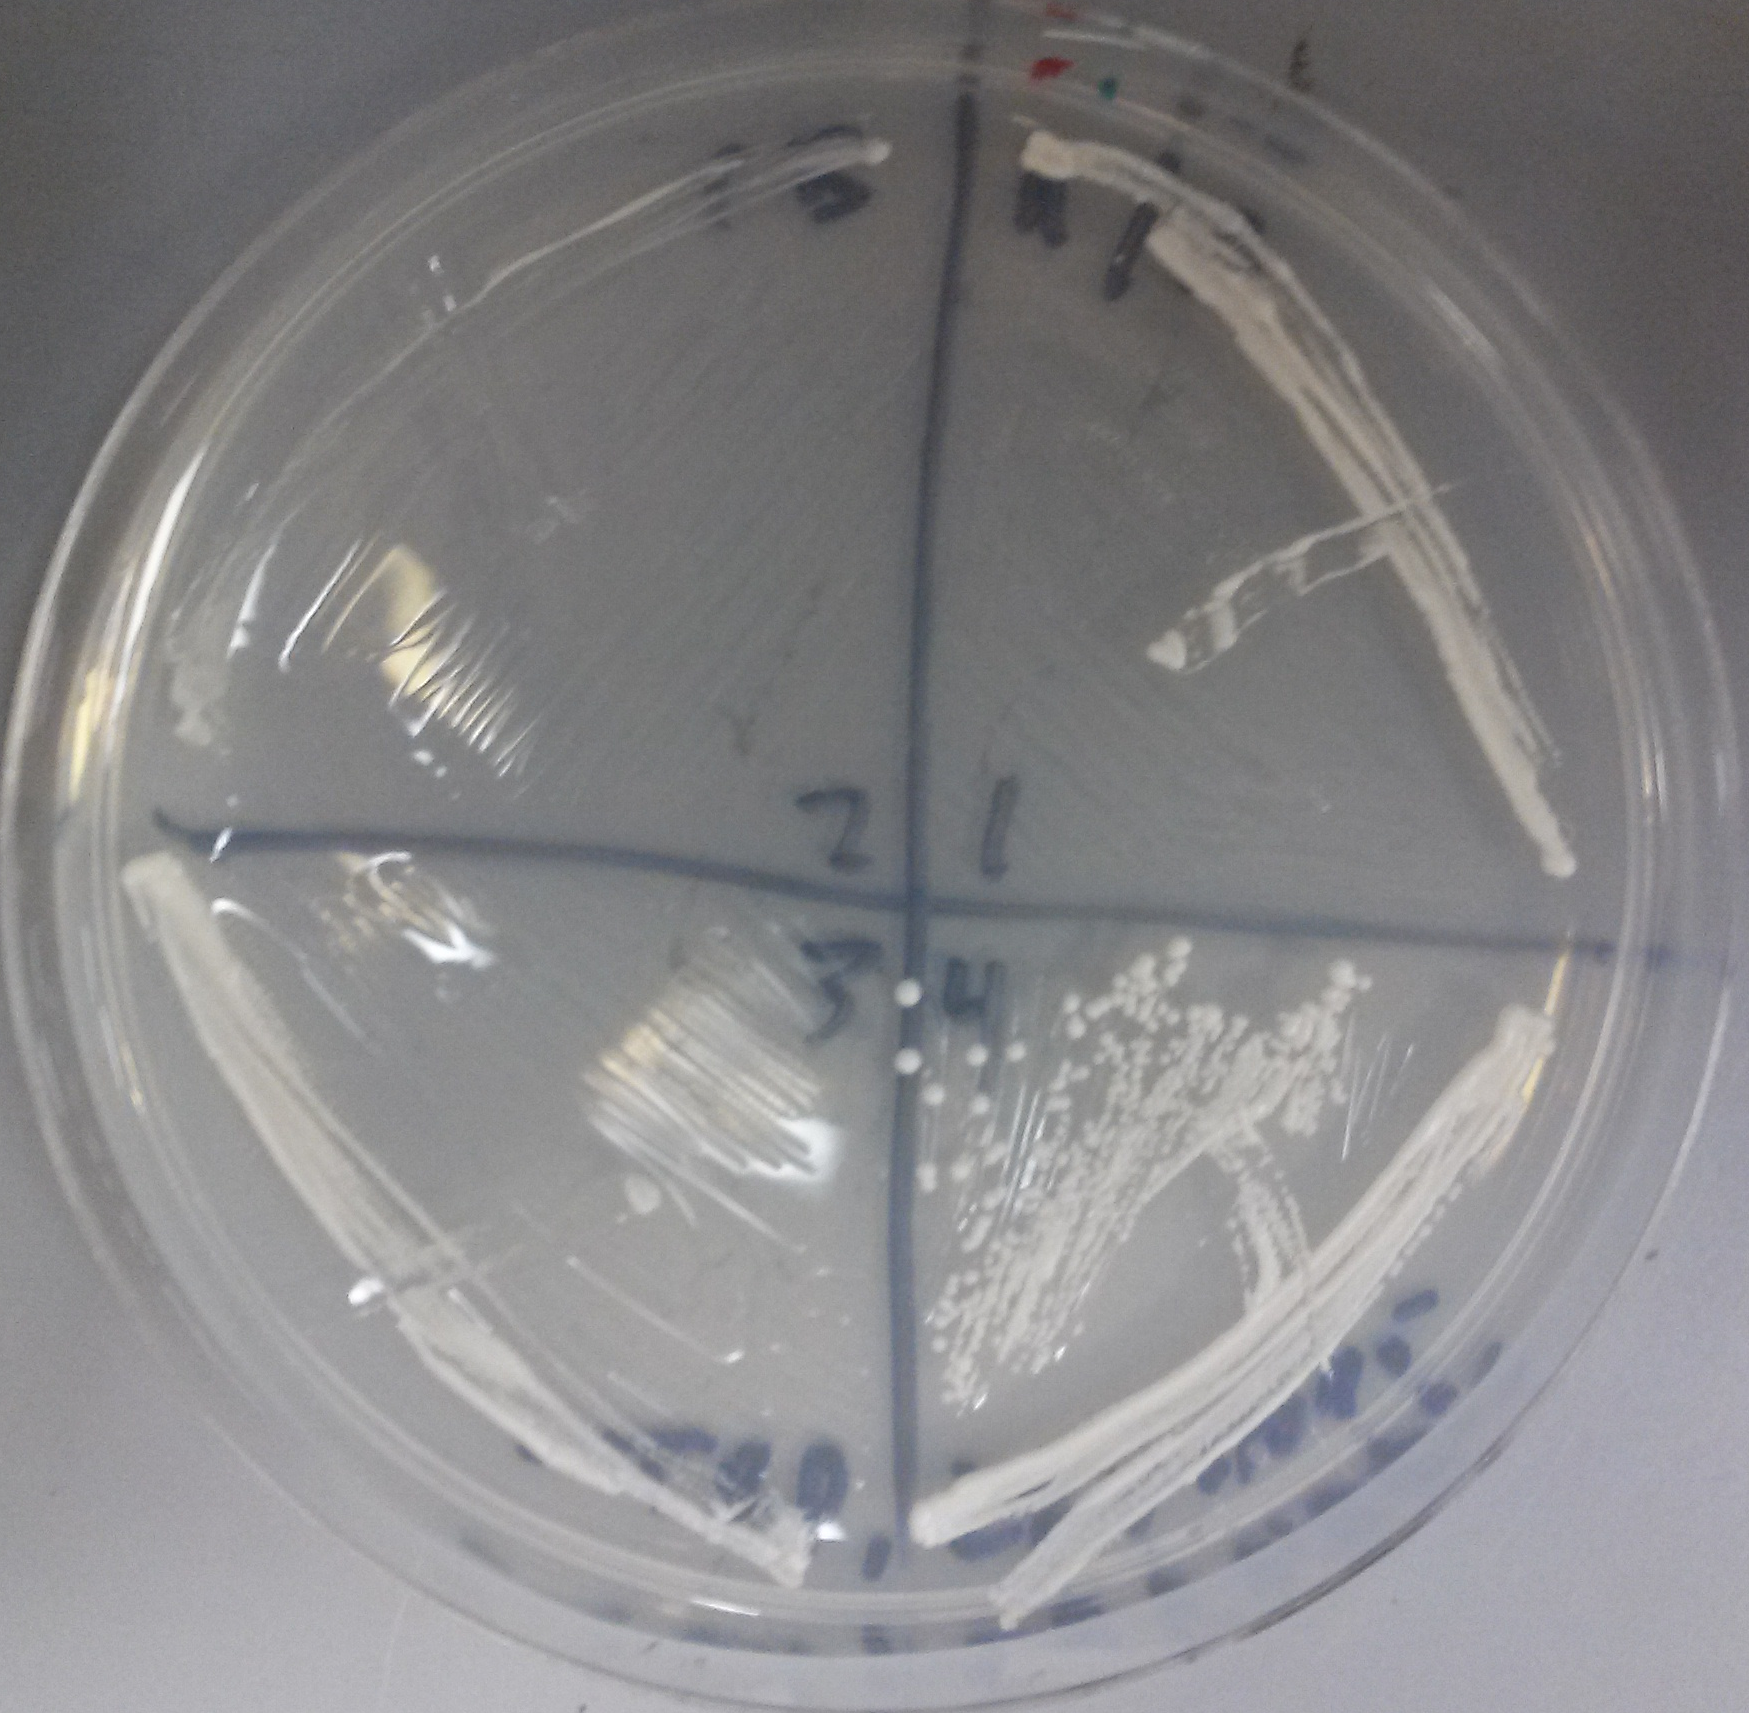
\includegraphics[width=.8\textwidth]{TRPstreak1118.png}
        \caption{TRP- streak on 11/18\\ After 2 days.}
        \label{fig:urastreak}
    \end{figure}
    \end{minipage}
        \hfill
    \begin{minipage}[ht!]{0.48\textwidth}
    \begin{figure}[ht!]
        \centering
        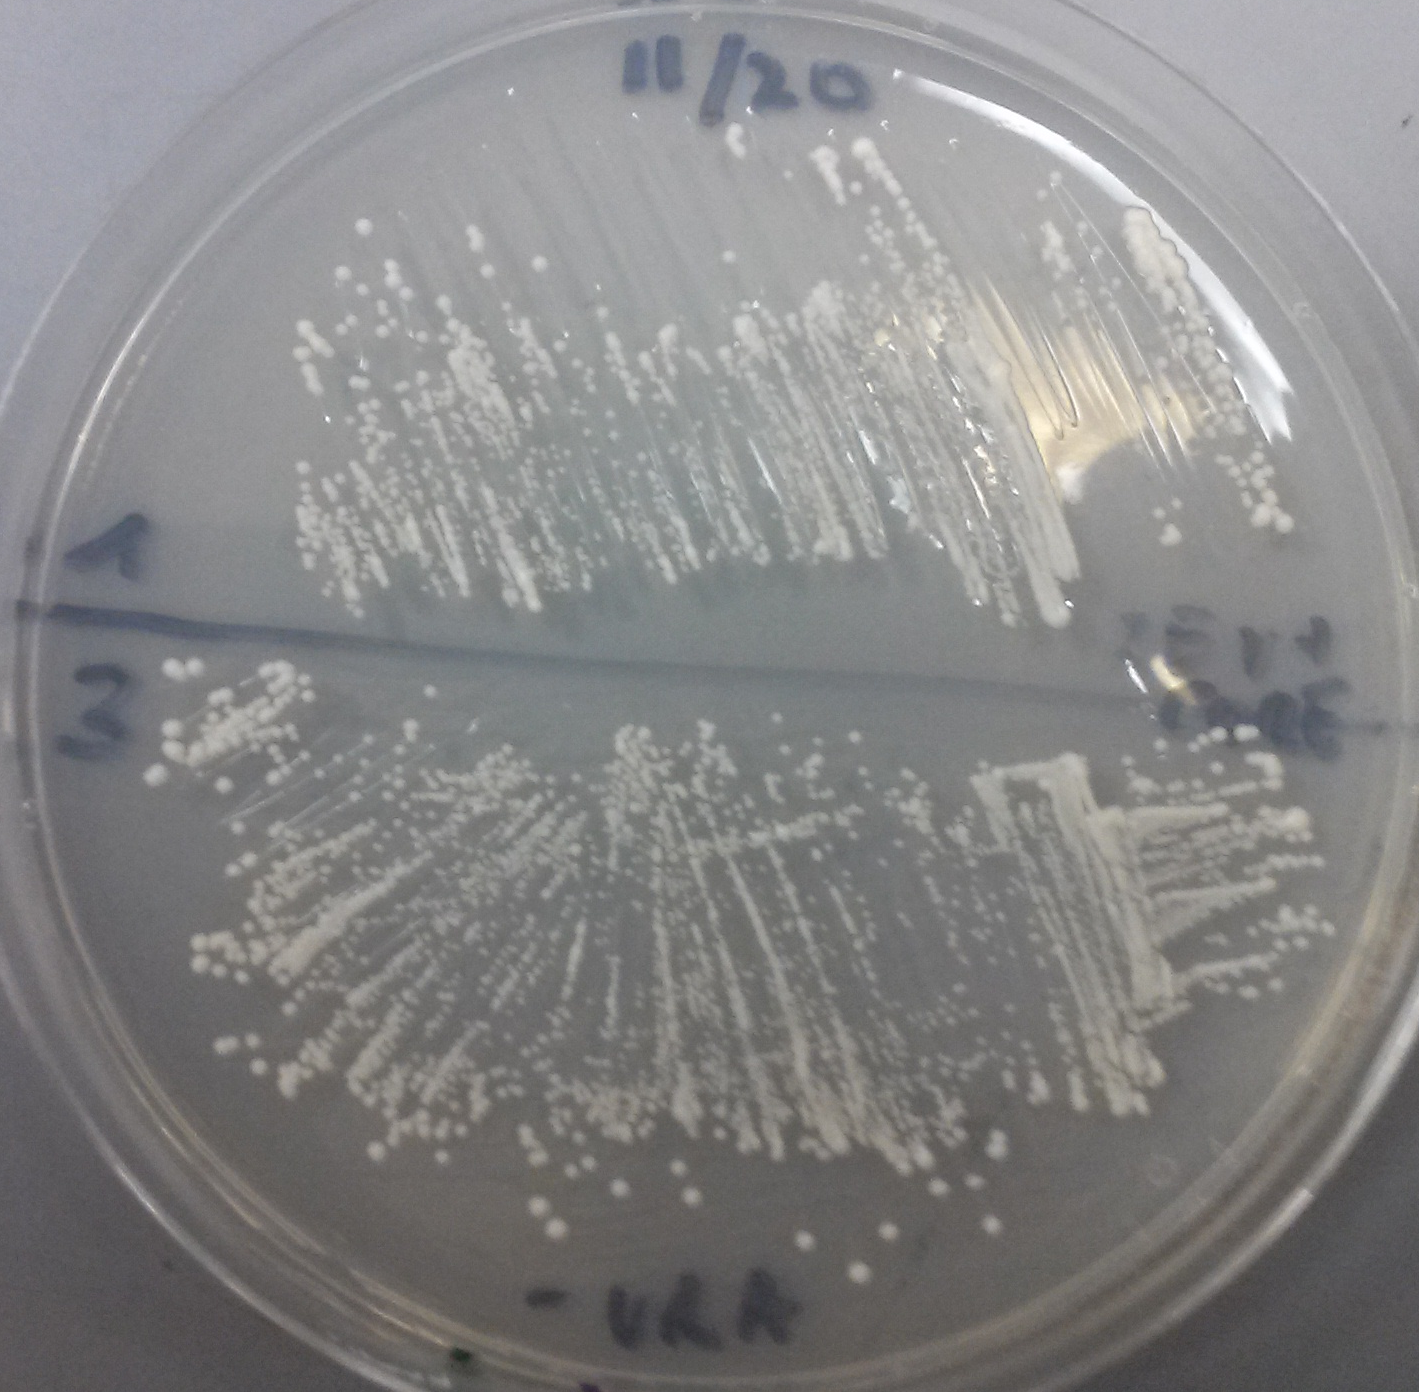
\includegraphics[width=.8\textwidth]{URAstreak1120.png}
        \caption{URA- streak on 11/20\\ Grown 4 days!}
        \label{fig:urastreak}
    \end{figure}
    \end{minipage}
    \textbf{Genomic Construction:}
    \begin{itemize}
        \item Redo TRP knockout?
        \item Otherwise, transform ZEV + CORE with the ZEVpr and FAR.
    \end{itemize}

\end{frame}


\end{document}
